\documentclass[]{article}
\usepackage{lmodern}
\usepackage{amssymb,amsmath}
\usepackage{ifxetex,ifluatex}
\usepackage{fixltx2e} % provides \textsubscript
\ifnum 0\ifxetex 1\fi\ifluatex 1\fi=0 % if pdftex
  \usepackage[T1]{fontenc}
  \usepackage[utf8]{inputenc}
\else % if luatex or xelatex
  \ifxetex
    \usepackage{mathspec}
  \else
    \usepackage{fontspec}
  \fi
  \defaultfontfeatures{Ligatures=TeX,Scale=MatchLowercase}
\fi
% use upquote if available, for straight quotes in verbatim environments
\IfFileExists{upquote.sty}{\usepackage{upquote}}{}
% use microtype if available
\IfFileExists{microtype.sty}{%
\usepackage{microtype}
\UseMicrotypeSet[protrusion]{basicmath} % disable protrusion for tt fonts
}{}
\usepackage[margin=1in]{geometry}
\usepackage{hyperref}
\hypersetup{unicode=true,
            pdftitle={Trabalho Final - R para Iniciantes},
            pdfauthor={Maurílio Bonora Júnior},
            pdfborder={0 0 0},
            breaklinks=true}
\urlstyle{same}  % don't use monospace font for urls
\usepackage{color}
\usepackage{fancyvrb}
\newcommand{\VerbBar}{|}
\newcommand{\VERB}{\Verb[commandchars=\\\{\}]}
\DefineVerbatimEnvironment{Highlighting}{Verbatim}{commandchars=\\\{\}}
% Add ',fontsize=\small' for more characters per line
\usepackage{framed}
\definecolor{shadecolor}{RGB}{248,248,248}
\newenvironment{Shaded}{\begin{snugshade}}{\end{snugshade}}
\newcommand{\AlertTok}[1]{\textcolor[rgb]{0.94,0.16,0.16}{#1}}
\newcommand{\AnnotationTok}[1]{\textcolor[rgb]{0.56,0.35,0.01}{\textbf{\textit{#1}}}}
\newcommand{\AttributeTok}[1]{\textcolor[rgb]{0.77,0.63,0.00}{#1}}
\newcommand{\BaseNTok}[1]{\textcolor[rgb]{0.00,0.00,0.81}{#1}}
\newcommand{\BuiltInTok}[1]{#1}
\newcommand{\CharTok}[1]{\textcolor[rgb]{0.31,0.60,0.02}{#1}}
\newcommand{\CommentTok}[1]{\textcolor[rgb]{0.56,0.35,0.01}{\textit{#1}}}
\newcommand{\CommentVarTok}[1]{\textcolor[rgb]{0.56,0.35,0.01}{\textbf{\textit{#1}}}}
\newcommand{\ConstantTok}[1]{\textcolor[rgb]{0.00,0.00,0.00}{#1}}
\newcommand{\ControlFlowTok}[1]{\textcolor[rgb]{0.13,0.29,0.53}{\textbf{#1}}}
\newcommand{\DataTypeTok}[1]{\textcolor[rgb]{0.13,0.29,0.53}{#1}}
\newcommand{\DecValTok}[1]{\textcolor[rgb]{0.00,0.00,0.81}{#1}}
\newcommand{\DocumentationTok}[1]{\textcolor[rgb]{0.56,0.35,0.01}{\textbf{\textit{#1}}}}
\newcommand{\ErrorTok}[1]{\textcolor[rgb]{0.64,0.00,0.00}{\textbf{#1}}}
\newcommand{\ExtensionTok}[1]{#1}
\newcommand{\FloatTok}[1]{\textcolor[rgb]{0.00,0.00,0.81}{#1}}
\newcommand{\FunctionTok}[1]{\textcolor[rgb]{0.00,0.00,0.00}{#1}}
\newcommand{\ImportTok}[1]{#1}
\newcommand{\InformationTok}[1]{\textcolor[rgb]{0.56,0.35,0.01}{\textbf{\textit{#1}}}}
\newcommand{\KeywordTok}[1]{\textcolor[rgb]{0.13,0.29,0.53}{\textbf{#1}}}
\newcommand{\NormalTok}[1]{#1}
\newcommand{\OperatorTok}[1]{\textcolor[rgb]{0.81,0.36,0.00}{\textbf{#1}}}
\newcommand{\OtherTok}[1]{\textcolor[rgb]{0.56,0.35,0.01}{#1}}
\newcommand{\PreprocessorTok}[1]{\textcolor[rgb]{0.56,0.35,0.01}{\textit{#1}}}
\newcommand{\RegionMarkerTok}[1]{#1}
\newcommand{\SpecialCharTok}[1]{\textcolor[rgb]{0.00,0.00,0.00}{#1}}
\newcommand{\SpecialStringTok}[1]{\textcolor[rgb]{0.31,0.60,0.02}{#1}}
\newcommand{\StringTok}[1]{\textcolor[rgb]{0.31,0.60,0.02}{#1}}
\newcommand{\VariableTok}[1]{\textcolor[rgb]{0.00,0.00,0.00}{#1}}
\newcommand{\VerbatimStringTok}[1]{\textcolor[rgb]{0.31,0.60,0.02}{#1}}
\newcommand{\WarningTok}[1]{\textcolor[rgb]{0.56,0.35,0.01}{\textbf{\textit{#1}}}}
\usepackage{graphicx,grffile}
\makeatletter
\def\maxwidth{\ifdim\Gin@nat@width>\linewidth\linewidth\else\Gin@nat@width\fi}
\def\maxheight{\ifdim\Gin@nat@height>\textheight\textheight\else\Gin@nat@height\fi}
\makeatother
% Scale images if necessary, so that they will not overflow the page
% margins by default, and it is still possible to overwrite the defaults
% using explicit options in \includegraphics[width, height, ...]{}
\setkeys{Gin}{width=\maxwidth,height=\maxheight,keepaspectratio}
\IfFileExists{parskip.sty}{%
\usepackage{parskip}
}{% else
\setlength{\parindent}{0pt}
\setlength{\parskip}{6pt plus 2pt minus 1pt}
}
\setlength{\emergencystretch}{3em}  % prevent overfull lines
\providecommand{\tightlist}{%
  \setlength{\itemsep}{0pt}\setlength{\parskip}{0pt}}
\setcounter{secnumdepth}{0}
% Redefines (sub)paragraphs to behave more like sections
\ifx\paragraph\undefined\else
\let\oldparagraph\paragraph
\renewcommand{\paragraph}[1]{\oldparagraph{#1}\mbox{}}
\fi
\ifx\subparagraph\undefined\else
\let\oldsubparagraph\subparagraph
\renewcommand{\subparagraph}[1]{\oldsubparagraph{#1}\mbox{}}
\fi

%%% Use protect on footnotes to avoid problems with footnotes in titles
\let\rmarkdownfootnote\footnote%
\def\footnote{\protect\rmarkdownfootnote}

%%% Change title format to be more compact
\usepackage{titling}

% Create subtitle command for use in maketitle
\providecommand{\subtitle}[1]{
  \posttitle{
    \begin{center}\large#1\end{center}
    }
}

\setlength{\droptitle}{-2em}

  \title{Trabalho Final - R para Iniciantes}
    \pretitle{\vspace{\droptitle}\centering\huge}
  \posttitle{\par}
    \author{Maurílio Bonora Júnior}
    \preauthor{\centering\large\emph}
  \postauthor{\par}
      \predate{\centering\large\emph}
  \postdate{\par}
    \date{26/04/2019}


\begin{document}
\maketitle

\hypertarget{introducao}{%
\subsection{Introdução}\label{introducao}}

Sempre que vamos escrever um projeto ou relatório, somos bombardeados
por um gigantesca base de dados com artigos de relevância variável sobre
o determinado assunto. Organizar e escolher os melhores artigos dentre
essa imensidão de referências é uma dura tarefa, que muitas vezes pode
demandar um tempo que muitos pesquisadores não têm. Contudo, com o
advento do R e seus diversos pacotes, entre eles o ``Bibliometrix'',
essa tarefa de comparar artigos para escolher os melhores se tornou
muito mais fácil. Para exemplificar isso, foram escolhidos dois termos
para se começar a busca de arquivos em base de dados (Scopus). Tais
termos foram: ``TCR'' e ``Signalling''. Abaixo segue todo o procedimento
com os códigos e gráficos possíveis de se fazer com o pacote
``Bibliometrix''.

\hypertarget{requerimentos}{%
\subsection{Requerimentos}\label{requerimentos}}

Para a realização do trabalho, foram necessários alguns programas e
pacotes, dentre eles:

\begin{itemize}
\item
  O próprio R: garante toda a linguagem R para se trabalhar;
\item
  RStudio: um software com uma interface mais elegante e amigável ao
  usuário para ele conseguir trabalho;
\item
  Git: um sistema de controle de versão distribuído. Utilizado
  juntamente do Rmarkdown para se fazer o upload direto do trabalho para
  um repositório em nuvem (Github);
\item
  MikTex: programa necessário para a conversão do Script do Rmarkdown
  para PDf;
\item
  Pacote ``Rmarkdown'': converte scripts do R (mais especificamente do
  Rmarkdown) em uma variedade de formatos incluindo HTML, MS Word, PDF e
  Beamer. Além disso, o Rmarkdown consegue compilar os scripts em
  especíes de ``livros'' onde é possível colocar comentários, códigos
  fontes e a saída (resultado) do código do script;
\item
  Pacote ``Bibliometrix'': garante um conjunto de ferramentas muito útil
  para análises na área de cientometria e bibliometria;
\item
  Um arquivo Scopus.bib: arquivo baixado da base de dados Scopus com
  todas as informações de artigos escolhidos a partir das
  palavras-chaves selecionado.
\end{itemize}

\hypertarget{desenvolvimento}{%
\subsection{Desenvolvimento}\label{desenvolvimento}}

\hypertarget{carregamento-e-conversao-dos-dados}{%
\paragraph{Carregamento e Conversão dos
Dados}\label{carregamento-e-conversao-dos-dados}}

Após a instalação do R, RStudio, Miktex e Git (lembrando que é
necessário a criação de um diretório com o nome do trabalho no Git), é
necessário fazer o download dos pacotes ``Rmarkdown'' e
``Bibliometrix''.

Em seguida é necessário carregar o pacote ``Bibliometrix'':

\begin{Shaded}
\begin{Highlighting}[]
\KeywordTok{library}\NormalTok{(bibliometrix)}
\end{Highlighting}
\end{Shaded}

\begin{verbatim}
## To cite bibliometrix in publications, please use:
## 
## Aria, M. & Cuccurullo, C. (2017) bibliometrix: An R-tool for comprehensive science mapping analysis, Journal of Informetrics, 11(4), pp 959-975, Elsevier.
##                         
## 
## http:\\www.bibliometrix.org
## 
##                         
## To start with the shiny web-interface, please digit:
## biblioshiny()
\end{verbatim}

Já com o arquivo scopus.bib dentro da sua pasta de trabalho está na hora
de começar a preparar os dados para as análises. A primeira função que
será utilizada é ``read.Files'', que converte todos os arquivos de texto
de scopus.bib em um grande vetor de caracteres que chamaremos de D.

\begin{Shaded}
\begin{Highlighting}[]
\NormalTok{D<-}\KeywordTok{readFiles}\NormalTok{(}\StringTok{"scopus.bib"}\NormalTok{)}
\end{Highlighting}
\end{Shaded}

Esse grande objeto D pode então ser convertido em um DataFrame a partir
da função ``convert2df''.

\begin{Shaded}
\begin{Highlighting}[]
\NormalTok{M <-}\StringTok{ }\KeywordTok{convert2df}\NormalTok{(D, }\DataTypeTok{dbsource =} \StringTok{"scopus"}\NormalTok{, }\DataTypeTok{format =} \StringTok{"bibtex"}\NormalTok{)}
\end{Highlighting}
\end{Shaded}

\begin{verbatim}
## 
## Converting your scopus collection into a bibliographic dataframe
## 
## Articles extracted   100 
## Articles extracted   200 
## Articles extracted   300 
## Articles extracted   400 
## Articles extracted   500 
## Articles extracted   511 
## Done!
## 
## 
## Generating affiliation field tag AU_UN from C1:  Done!
\end{verbatim}

\hypertarget{analise-bibliometrica}{%
\paragraph{Análise Bibliométrica}\label{analise-bibliometrica}}

O primeiro passo para fazer uma análise descritiva desse Data Frame é
utilizara função ``biblioAnalysis'', que irá calcular as principais
medidas bibliométricas de toda nossa base de dados.

\begin{Shaded}
\begin{Highlighting}[]
\NormalTok{results<-}\KeywordTok{biblioAnalysis}\NormalTok{(M, }\DataTypeTok{sep =} \StringTok{";"}\NormalTok{)}
\end{Highlighting}
\end{Shaded}

Tal função retorna um objeto da classe bibliometrix (introduzida com o
pacote homônimo), que contem os seguintes componentes como o número
total de artigos, primeiro autor de cada manuscrito, número de vezes que
cada manustrico foi citado, entre outros. Para mais informações use a
função:

\begin{Shaded}
\begin{Highlighting}[]
\KeywordTok{help}\NormalTok{(}\StringTok{"biblioAnalysis"}\NormalTok{)}
\end{Highlighting}
\end{Shaded}

\begin{verbatim}
## starting httpd help server ... done
\end{verbatim}

Contudo, o objeto ``results'' que obtemos ainda é muito grande e
complicado de se ler, sendo muito laborioso obter informações gerais a
partir dali. Para isso, usa-se a função ``summary'' para se obter os
principais resultados da nossa análise bibliométrica. Essa função aceita
ainda dois argumentos adicionais: ``k'' é um valor de formatação que
indica quantas linhas de cada tabela serão mostradas, enquanto ``pause''
é um valor lógico usado para permitir ou não a pausa na rolagem da tela.

\begin{Shaded}
\begin{Highlighting}[]
\KeywordTok{summary}\NormalTok{(results, }\DataTypeTok{k =}\DecValTok{10}\NormalTok{, }\DataTypeTok{pause =} \OtherTok{FALSE}\NormalTok{)}
\end{Highlighting}
\end{Shaded}

\begin{verbatim}
## 
## 
## Main Information about data
## 
##  Documents                             511 
##  Sources (Journals, Books, etc.)       127 
##  Keywords Plus (ID)                    3213 
##  Author's Keywords (DE)                609 
##  Period                                1989 - 2019 
##  Average citations per documents       38.77 
## 
##  Authors                               2560 
##  Author Appearances                    3047 
##  Authors of single-authored documents  16 
##  Authors of multi-authored documents   2544 
##  Single-authored documents             17 
## 
##  Documents per Author                  0.2 
##  Authors per Document                  5.01 
##  Co-Authors per Documents              5.96 
##  Collaboration Index                   5.15 
##  
##  Document types                     
##  ARTICLE               445 
##  BOOK CHAPTER          6 
##  CONFERENCE PAPER      5 
##  EDITORIAL             2 
##  ERRATUM               4 
##  NOTE                  5 
##  REVIEW                40 
##  SHORT SURVEY          4 
##  
## 
## Annual Scientific Production
## 
##  Year    Articles
##     1989        1
##     1990        1
##     1991        1
##     1992        1
##     1993        3
##     1994        7
##     1995        4
##     1996       10
##     1997       21
##     1998       30
##     1999       25
##     2000       21
##     2001       23
##     2002       24
##     2003       21
##     2004       15
##     2005       23
##     2006       16
##     2007       18
##     2008       20
##     2009       12
##     2010       14
##     2011       23
##     2012       26
##     2013       19
##     2014       27
##     2015       24
##     2016       18
##     2017       23
##     2018       31
##     2019        9
## 
## Annual Percentage Growth Rate 7.598962 
## 
## 
## Most Productive Authors
## 
##    Authors        Articles Authors        Articles Fractionalized
## 1     WEISS A           11    SAMELSON LE                    2.52
## 2     SAMELSON LE       10    WEISS A                        2.42
## 3     LOVE PE            9    ACUTO O                        2.21
## 4     SCHRAVEN B         9    NA NA                          2.00
## 5     ACUTO O            8    HARDER T                       1.81
## 6     SIMEONI L          7    ABRAHAM RT                     1.70
## 7     ZHANG W            7    WANGE RL                       1.64
## 8     BALDARI CT         6    LOVE PE                        1.61
## 9     CARPINO N          6    MICHEL F                       1.60
## 10    LI Y               6    SCHRAVEN B                     1.58
## 
## 
## Top manuscripts per citations
## 
##                    Paper           TC TCperYear
## 1  MERESSE B, 2004, IMMUNITY      545     36.33
## 2  WANGE RL, 1996, IMMUNITY       443     19.26
## 3  ACUTO O, 2003, NAT REV IMMUNOL 413     25.81
## 4  MOSSMAN KD, 2005, SCIENCE      361     25.79
## 5  DOWER NA, 2000, NAT IMMUNOL    334     17.58
## 6  JANES PW, 2000, SEMIN IMMUNOL  322     16.95
## 7  KERSH GJ, 1998, IMMUNITY       248     11.81
## 8  KRAUSE M, 2000, J CELL BIOL    240     12.63
## 9  ZHANG W, 1999, INT IMMUNOL     218     10.90
## 10 CHAN AC, 1994, J IMMUNOL       218      8.72
## 
## 
## Corresponding Author's Countries
## 
##           Country Articles   Freq SCP MCP MCP_Ratio
## 1  USA                 208 0.4771 179  29     0.139
## 2  FRANCE               29 0.0665  19  10     0.345
## 3  GERMANY              28 0.0642  15  13     0.464
## 4  UNITED KINGDOM       28 0.0642  17  11     0.393
## 5  JAPAN                18 0.0413  15   3     0.167
## 6  CANADA               16 0.0367   9   7     0.438
## 7  SWITZERLAND          16 0.0367  11   5     0.312
## 8  ITALY                14 0.0321   8   6     0.429
## 9  KOREA                12 0.0275  10   2     0.167
## 10 CHINA                11 0.0252   7   4     0.364
## 
## 
## SCP: Single Country Publications
## 
## MCP: Multiple Country Publications
## 
## 
## Total Citations per Country
## 
##      Country      Total Citations Average Article Citations
## 1  USA                      10614                     51.03
## 2  FRANCE                    1619                     55.83
## 3  UNITED KINGDOM            1461                     52.18
## 4  GERMANY                   1046                     37.36
## 5  CANADA                    1032                     64.50
## 6  JAPAN                      660                     36.67
## 7  SWITZERLAND                597                     37.31
## 8  ITALY                      529                     37.79
## 9  NETHERLANDS                397                     56.71
## 10 AUSTRALIA                  278                     34.75
## 
## 
## Most Relevant Sources
## 
##                      Sources        Articles
## 1  JOURNAL OF IMMUNOLOGY                 158
## 2  EUROPEAN JOURNAL OF IMMUNOLOGY         32
## 3  NATURE IMMUNOLOGY                      26
## 4  BLOOD                                  16
## 5  JOURNAL OF EXPERIMENTAL MEDICINE       16
## 6  FRONTIERS IN IMMUNOLOGY                14
## 7  IMMUNITY                               14
## 8  INTERNATIONAL IMMUNOLOGY               14
## 9  MOLECULAR IMMUNOLOGY                   14
## 10 PLOS ONE                                9
## 
## 
## Most Relevant Keywords
## 
##    Author Keywords (DE)      Articles Keywords-Plus (ID)     Articles
## 1        SIGNAL TRANSDUCTION       28  SIGNAL TRANSDUCTION        788
## 2        TCR                       27  MICE                       477
## 3        TCR SIGNALING             18  RECEPTORS                  420
## 4        T CELL RECEPTOR           17  ARTICLE                    418
## 5        T LYMPHOCYTES             16  T LYMPHOCYTE RECEPTOR      402
## 6        T CELL                    15  ANTIGEN                    400
## 7        T CELL ACTIVATION         15  T CELL                     397
## 8        T CELLS                   14  PRIORITY JOURNAL           380
## 9        SIGNALING                 11  HUMAN                      315
## 10       T CELL SIGNALING          10  MOUSE                      314
\end{verbatim}

A partir daí obtemos uma série de resultados interessantes, desde as
principais informações dos nossos dados - como nº de documentos, média
de citações por artigos, nº de autores, nº de artigos com autores únicos
- até informações mais curiosas como a produção de artios por ano desde
o primeiro que foi publicado, autores mais produtivos, países com
maiores nº de citações, principais fontes de artigos, entre diversas
outras. Por fim, a partir dessas mesmos informações básicas obtidas, é
possível montar gráficos que nos dão uma ideia bem mais visual da
relação entre nossos dados, usando a função ``plot''.

\begin{Shaded}
\begin{Highlighting}[]
\KeywordTok{plot}\NormalTok{(}\DataTypeTok{x=}\NormalTok{results, }\DataTypeTok{k=}\DecValTok{10}\NormalTok{, }\DataTypeTok{pause=}\OtherTok{FALSE}\NormalTok{)}
\end{Highlighting}
\end{Shaded}

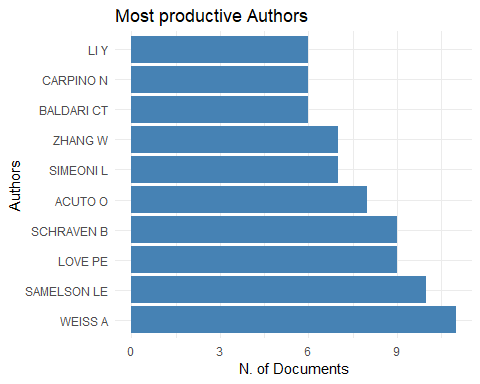
\includegraphics{Primeiro_Script_files/figure-latex/unnamed-chunk-7-1.pdf}
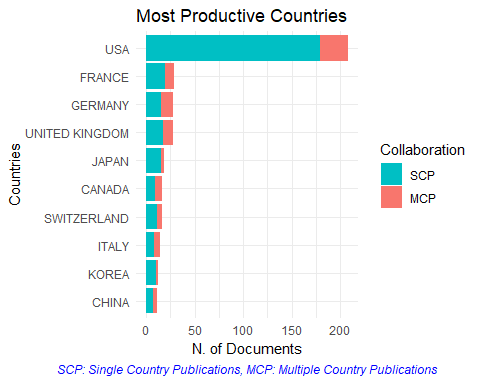
\includegraphics{Primeiro_Script_files/figure-latex/unnamed-chunk-7-2.pdf}
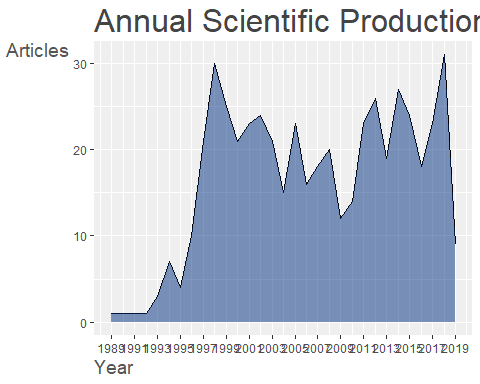
\includegraphics{Primeiro_Script_files/figure-latex/unnamed-chunk-7-3.pdf}
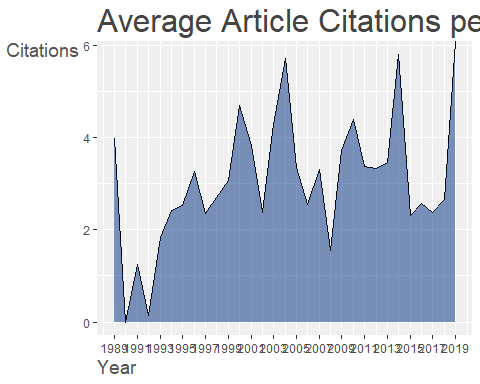
\includegraphics{Primeiro_Script_files/figure-latex/unnamed-chunk-7-4.pdf}
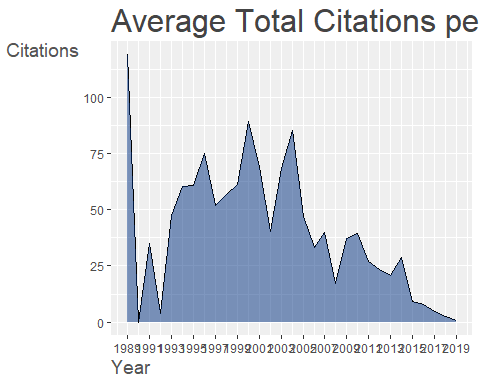
\includegraphics{Primeiro_Script_files/figure-latex/unnamed-chunk-7-5.pdf}

\hypertarget{analise-de-referencias-citadas}{%
\paragraph{Análise de Referências
Citadas}\label{analise-de-referencias-citadas}}

É possível produzir uma tabela mostrando as referências mais citadas dos
autores mais citados, utilizando-se a função ``citations''. Para se
obter os artigos mais citadas, usa-se:

\begin{Shaded}
\begin{Highlighting}[]
\NormalTok{CR <-}\StringTok{ }\KeywordTok{citations}\NormalTok{(M, }\DataTypeTok{field =} \StringTok{"article"}\NormalTok{, }\DataTypeTok{sep =} \StringTok{";"}\NormalTok{)}
\KeywordTok{cbind}\NormalTok{(CR}\OperatorTok{$}\NormalTok{Cited[}\DecValTok{1}\OperatorTok{:}\DecValTok{10}\NormalTok{])}
\end{Highlighting}
\end{Shaded}

\begin{verbatim}
##                                                                                                                                                                                                                                          [,1]
## ZHANG, W., SLOAN-LANCASTER, J., KITCHEN, J., TRIBLE, R.P., SAMELSON, L.E., LAT: THE ZAP-70 TYROSINE KINASE SUBSTRATE THAT LINKS T CELL RECEPTOR TO CELLULAR ACTIVATION (1998) CELL, 92, PP. 83-92                                          24
## SMITH-GARVIN, J.E., KORETZKY, G.A., JORDAN, M.S., T CELL ACTIVATION (2009) ANNU. REV. IMMUNOL., 27, PP. 591-619                                                                                                                            21
## WEISS, A., LITTMAN, D.R., SIGNAL TRANSDUCTION BY LYMPHOCYTE ANTIGEN RECEPTORS (1994) CELL, 76, PP. 263-274                                                                                                                                 20
## WEISS, A., LITTMAN, D.R., SIGNAL TRANSDUCTION BY LYMPHOCYTE ANTIGEN RECEPTORS (1994) CELL, 76, P. 263                                                                                                                                      16
## XAVIER, R., BRENNAN, T., LI, Q., MCCORMACK, C., SEED, B., MEMBRANE COMPARTMENTATION IS REQUIRED FOR EFFICIENT T CELL ACTIVATION (1998) IMMUNITY, 8, PP. 723-732                                                                            13
## VARMA, R., CAMPI, G., YOKOSUKA, T., SAITO, T., DUSTIN, M.L., T CELL RECEPTOR-PROXIMAL SIGNALS ARE SUSTAINED IN PERIPHERAL MICROCLUSTERS AND TERMINATED IN THE CENTRAL SUPRAMOLECULAR ACTIVATION CLUSTER (2006) IMMUNITY, 25, PP. 117-127   12
## VIOLA, A., SCHROEDER, S., SAKAKIBARA, Y., LANZAVECCHIA, A., T LYMPHOCYTE COSTIMULATION MEDIATED BY REORGANIZATION OF MEMBRANE MICRODOMAINS (1999) SCIENCE, 283, PP. 680-682                                                                12
## WANGE, R.L., SAMELSON, L.E., COMPLEX COMPLEXES: SIGNALING AT THE TCR (1996) IMMUNITY, 5, P. 197                                                                                                                                            11
## ZHANG, W., TRIBLE, R.P., SAMELSON, L.E., LAT PALMITOYLATION: ITS ESSENTIAL ROLE IN MEMBRANE MICRODOMAIN TARGETING AND TYROSINE PHOSPHORYLATION DURING T CELL ACTIVATION (1998) IMMUNITY, 9, PP. 239-246                                    11
## CANTRELL, D., T CELL ANTIGEN RECEPTOR SIGNAL TRANSDUCTION PATHWAYS (1996) ANNU. REV. IMMUNOL., 14, P. 259                                                                                                                                  10
\end{verbatim}

Enquanto que para se obter os autores mais citados, usa-se:

\begin{Shaded}
\begin{Highlighting}[]
\NormalTok{CR<-}\StringTok{ }\KeywordTok{citations}\NormalTok{(M, }\DataTypeTok{field =} \StringTok{"author"}\NormalTok{, }\DataTypeTok{sep =} \StringTok{";"}\NormalTok{)}
\KeywordTok{cbind}\NormalTok{(CR}\OperatorTok{$}\NormalTok{Cited[}\DecValTok{1}\OperatorTok{:}\DecValTok{10}\NormalTok{])}
\end{Highlighting}
\end{Shaded}

\begin{verbatim}
##               [,1]
## WEISS A        669
## SAMELSON L E   403
## KORETZKY G A   268
## DAVIS M M      244
## VON BOEHMER H  240
## CHAN A C       219
## ZHANG W        216
## GERMAIN R N    192
## ALLEN P M      185
## DUSTIN M L     177
\end{verbatim}

Por fim, é possível montar ainda uma tabela onde mostra-se os autores
mais citados ``localmente'', isto é, dentre a base de dados que temos,
quais foram os autores mais citados entre os outros autores dessa base.
Para isso, utilizamos a função ``LocalCitations''. Utilizaremos as
mesmas funções auxiliares usadas anteriormente para ver os 10 principais
autores e principais artigos citados local e respectivamente:

\begin{Shaded}
\begin{Highlighting}[]
\NormalTok{CR <-}\StringTok{ }\KeywordTok{localCitations}\NormalTok{(M, }\DataTypeTok{sep =} \StringTok{";"}\NormalTok{)}
\end{Highlighting}
\end{Shaded}

\begin{verbatim}
## Articles analysed   100 
## Articles analysed   200 
## Articles analysed   300 
## Articles analysed   400 
## Articles analysed   462
\end{verbatim}

\begin{Shaded}
\begin{Highlighting}[]
\NormalTok{CR}\OperatorTok{$}\NormalTok{Authors[}\DecValTok{1}\OperatorTok{:}\DecValTok{10}\NormalTok{,]}
\end{Highlighting}
\end{Shaded}

\begin{verbatim}
##                Author LocalCitations
## 11            ACUTO O             30
## 1776      SAMELSON LE             28
## 1389         MICHEL F             21
## 2213         WANGE RL             21
## 1255          LOVE PE             20
## 2121         TUOSTO L             16
## 88   ATTAL BONNEFOY G             14
## 1302        MANGINO G             14
## 2227          WEISS A             14
## 1896        SHORES EW             13
\end{verbatim}

\begin{Shaded}
\begin{Highlighting}[]
\NormalTok{CR}\OperatorTok{$}\NormalTok{Papers[}\DecValTok{1}\OperatorTok{:}\DecValTok{10}\NormalTok{,]}
\end{Highlighting}
\end{Shaded}

\begin{verbatim}
##                             Paper                                                                DOI Year LCS GCS
## 24       WANGE RL, 1996, IMMUNITY                                      10.1016/S1074-7613(00)80315-5 1996  19 443
## 58  TUOSTO L, 1998, EUR J IMMUNOL 10.1002/(SICI)1521-4141(199807)28:07<2131::AID-IMMU2131>3.0.CO;2-Q 1998   9  85
## 124     AZZAM HS, 2001, J IMMUNOL                                        10.4049/JIMMUNOL.166.9.5464 2001   9 180
## 191    CIOFANI M, 2004, J IMMUNOL                                        10.4049/JIMMUNOL.172.9.5230 2004   9 183
## 99      MICHEL F, 2000, J IMMUNOL                                        10.4049/JIMMUNOL.165.7.3820 2000   7  73
## 132      MICHEL F, 2001, IMMUNITY                                      10.1016/S1074-7613(01)00244-8 2001   7 128
## 133        RAAB M, 2001, IMMUNITY                                      10.1016/S1074-7613(01)00248-5 2001   7  84
## 362     GUY CS, 2013, NAT IMMUNOL                                                    10.1038/NI.2538 2013   7  97
## 139      KOSUGI A, 2001, IMMUNITY                                      10.1016/S1074-7613(01)00146-7 2001   6  85
## 195     CARPINO N, 2004, IMMUNITY                                      10.1016/S1074-7613(03)00351-0 2004   6 100
\end{verbatim}

\hypertarget{ranking-de-dominancia-de-autores}{%
\paragraph{Ranking de Dominância de
Autores}\label{ranking-de-dominancia-de-autores}}

O fator de dominância é uma taxa que indica a fração de artigos com
múltiplos autores em que um pesquisador aparece como primeiro autor. A
função ``dominance'' calcula o ranking da dominância entre os autores.

\begin{Shaded}
\begin{Highlighting}[]
\NormalTok{DF <-}\StringTok{ }\KeywordTok{dominance}\NormalTok{(results, }\DataTypeTok{k =} \DecValTok{10}\NormalTok{)}
\NormalTok{DF}
\end{Highlighting}
\end{Shaded}

\begin{verbatim}
##          Author Dominance Factor Tot Articles Single-Authored Multi-Authored First-Authored Rank by Articles Rank by DF
## 1      HARDER T        0.6666667            4               1              3              2                1          1
## 2      MICHEL F        0.5000000            6               0              6              3                5          2
## 3     CARPINO N        0.3333333            6               0              6              2                5          3
## 4   HOUTMAN JCD        0.2500000            4               0              4              1                1          4
## 5  LEITENBERG D        0.2500000            4               0              4              1                1          4
## 6  VAN OERS NSC        0.2000000            5               0              5              1                4          6
## 7          LI Y        0.1666667            6               0              6              1                5          7
## 8       ZHANG W        0.1428571            7               0              7              1                8          8
## 9       ACUTO O        0.1250000            8               0              8              1                9          9
## 10      LOVE PE        0.1111111            9               0              9              1               10         10
\end{verbatim}

\hypertarget{o-indice-h-dos-autores}{%
\paragraph{O índice-h dos autores}\label{o-indice-h-dos-autores}}

O índice-h é uma métrica que mede ambas produtividade e impacto de
citação das publicações de cientistas. Esse índice é baseado no conjunto
de artigos mais citados do autor em específico e no número de citações
que esses artigos receberam em outras publicações. A função ``Hindex''
calcula o índice-h de autores ou de fontes e suas variantes (índice-g e
índice-m) em uma conjunto de dados bibliográficos. Para calcular o
índice-h dos 10 autores mais produtivos dessa coleção em específico,
utilizaremos os seguintes códigos:

\begin{Shaded}
\begin{Highlighting}[]
\NormalTok{authors=}\KeywordTok{gsub}\NormalTok{(}\StringTok{","}\NormalTok{,}\StringTok{" "}\NormalTok{,}\KeywordTok{names}\NormalTok{(results}\OperatorTok{$}\NormalTok{Authors)[}\DecValTok{1}\OperatorTok{:}\DecValTok{10}\NormalTok{])}
\NormalTok{indices <-}\StringTok{ }\KeywordTok{Hindex}\NormalTok{(M, }\DataTypeTok{field =} \StringTok{"author"}\NormalTok{, }\DataTypeTok{elements=}\NormalTok{authors, }\DataTypeTok{sep =} \StringTok{";"}\NormalTok{, }\DataTypeTok{years =} \DecValTok{50}\NormalTok{)}
\NormalTok{indices}\OperatorTok{$}\NormalTok{H}
\end{Highlighting}
\end{Shaded}

\begin{verbatim}
##         Author h_index g_index   m_index  TC NP PY_start
## 1      WEISS A      10      11 0.3846154 819 11     1994
## 2  SAMELSON LE       8      10 0.3333333 907 10     1996
## 3      LOVE PE       7       9 0.3043478 471  9     1997
## 4   SCHRAVEN B       7       9 0.3181818 222  9     1998
## 5      ACUTO O       8       8 0.3636364 905  8     1998
## 6    SIMEONI L       4       7 0.2352941  69  7     2003
## 7      ZHANG W       4       7 0.1904762 319  7     1999
## 8   BALDARI CT       5       6 0.2500000 174  6     2000
## 9    CARPINO N       4       6 0.2500000 197  6     2004
## 10        LI Y       5       8 0.3333333 177  8     2005
\end{verbatim}

\hypertarget{produtividade-dos-principais-autores-no-decorrer-do-tempo}{%
\paragraph{Produtividade dos principais autores no decorrer do
tempo}\label{produtividade-dos-principais-autores-no-decorrer-do-tempo}}

A função ``AuthorProdOverTime'' facilmente consegue nos dar um gráfico
mostrando a produção dos 10 primeiros autores (em termos de número de
publicações e número de citações totais por ano) no decorrer do tempo.

\begin{Shaded}
\begin{Highlighting}[]
\NormalTok{topAU <-}\StringTok{ }\KeywordTok{authorProdOverTime}\NormalTok{(M, }\DataTypeTok{k =} \DecValTok{10}\NormalTok{, }\DataTypeTok{graph =} \OtherTok{TRUE}\NormalTok{)}
\end{Highlighting}
\end{Shaded}

\includegraphics{Primeiro_Script_files/figure-latex/unnamed-chunk-13-1.pdf}

\hypertarget{estimativa-do-coeficiente-da-regra-de-lotka}{%
\paragraph{Estimativa do coeficiente da regra de
Lotka}\label{estimativa-do-coeficiente-da-regra-de-lotka}}

A regra de Lotka descreve a frequência de publicação dos autores de um
determinado campo como uma lei do quadrado inversa, onde o número de
autores publicando um determinado número de artigos é uma taxa fixa para
o número de autores publicando um artigo único. Essa suposição implica
que o coeficiente beta teórico da regra de Lotka é igual a 2. A função
``lotka'' estima os coeficientes dessa regra de Lotka. Usando tal função
é possível estimar por exemplo o coeficiente beta, dito anteriormente,
de nossa coleção bibliográfica e acessar - a partir de um teste
estatístico - a similaridade da distribuição empírica com uma teórica.

\begin{itemize}
\tightlist
\item
  Distribuição empírica da produtividade dos autores:
\end{itemize}

\begin{Shaded}
\begin{Highlighting}[]
\NormalTok{L <-}\StringTok{ }\KeywordTok{lotka}\NormalTok{(results)}
\NormalTok{L}\OperatorTok{$}\NormalTok{AuthorProd}
\end{Highlighting}
\end{Shaded}

\begin{verbatim}
##    N.Articles N.Authors        Freq
## 1           1      2248 0.878125000
## 2           2       224 0.087500000
## 3           3        48 0.018750000
## 4           4        23 0.008984375
## 5           5         6 0.002343750
## 6           6         4 0.001562500
## 7           7         2 0.000781250
## 8           8         1 0.000390625
## 9           9         2 0.000781250
## 10         10         1 0.000390625
## 11         11         1 0.000390625
\end{verbatim}

\begin{itemize}
\tightlist
\item
  Coeficiente beta estimado:
\end{itemize}

\begin{Shaded}
\begin{Highlighting}[]
\NormalTok{L}\OperatorTok{$}\NormalTok{Beta}
\end{Highlighting}
\end{Shaded}

\begin{verbatim}
## [1] 3.370245
\end{verbatim}

\begin{itemize}
\tightlist
\item
  Constante:
\end{itemize}

\begin{Shaded}
\begin{Highlighting}[]
\NormalTok{L}\OperatorTok{$}\NormalTok{C}
\end{Highlighting}
\end{Shaded}

\begin{verbatim}
## [1] 0.7867831
\end{verbatim}

\begin{itemize}
\tightlist
\item
  Qualidade de ajuste:
\end{itemize}

\begin{Shaded}
\begin{Highlighting}[]
\NormalTok{L}\OperatorTok{$}\NormalTok{R2}
\end{Highlighting}
\end{Shaded}

\begin{verbatim}
## [1] 0.980799
\end{verbatim}

\begin{itemize}
\tightlist
\item
  Valor p dos dois testes K-S da amostra
\end{itemize}

\begin{Shaded}
\begin{Highlighting}[]
\NormalTok{L}\OperatorTok{$}\NormalTok{p.value}
\end{Highlighting}
\end{Shaded}

\begin{verbatim}
## [1] 0.02325117
\end{verbatim}

A tabela L\$AuthorProd mostra a distribuição da produção científica
observada em nosso exemplo. Nosso coeficiente beta é de aproximadamente
3.3 com uma qualiidade de ajuste de 0.98. Os dois testes (estatísticos)
Kolmogorov-Smirnoff nos provê um valor p de 0.02, o que significa que
basicamente não há diferença estatística entre nossos distribuições
Lotka esperada e observada. Para uma visão gráfica disso, é possível
usar a função plot:

\begin{Shaded}
\begin{Highlighting}[]
\NormalTok{Observed=L}\OperatorTok{$}\NormalTok{AuthorProd[,}\DecValTok{3}\NormalTok{]}
\NormalTok{Theoretical=}\DecValTok{10}\OperatorTok{^}\NormalTok{(}\KeywordTok{log10}\NormalTok{(L}\OperatorTok{$}\NormalTok{C)}\OperatorTok{-}\DecValTok{2}\OperatorTok{*}\KeywordTok{log10}\NormalTok{(L}\OperatorTok{$}\NormalTok{AuthorProd[,}\DecValTok{1}\NormalTok{]))}
\KeywordTok{plot}\NormalTok{(L}\OperatorTok{$}\NormalTok{AuthorProd[,}\DecValTok{1}\NormalTok{],Theoretical,}\DataTypeTok{type=}\StringTok{"l"}\NormalTok{,}\DataTypeTok{col=}\StringTok{"red"}\NormalTok{,}\DataTypeTok{ylim=}\KeywordTok{c}\NormalTok{(}\DecValTok{0}\NormalTok{, }\DecValTok{1}\NormalTok{), }\DataTypeTok{xlab=}\StringTok{"Articles"}\NormalTok{,}\DataTypeTok{ylab=}\StringTok{"Freq. of Authors"}\NormalTok{,}\DataTypeTok{main=}\StringTok{"Scientific Productivity"}\NormalTok{)}
\KeywordTok{lines}\NormalTok{(L}\OperatorTok{$}\NormalTok{AuthorProd[,}\DecValTok{1}\NormalTok{],Observed,}\DataTypeTok{col=}\StringTok{"blue"}\NormalTok{)}
\KeywordTok{legend}\NormalTok{(}\DataTypeTok{x=}\StringTok{"topright"}\NormalTok{,}\KeywordTok{c}\NormalTok{(}\StringTok{"Theoretical (B=2)"}\NormalTok{,}\StringTok{"Observed"}\NormalTok{),}\DataTypeTok{col=}\KeywordTok{c}\NormalTok{(}\StringTok{"red"}\NormalTok{,}\StringTok{"blue"}\NormalTok{),}\DataTypeTok{lty =} \KeywordTok{c}\NormalTok{(}\DecValTok{1}\NormalTok{,}\DecValTok{1}\NormalTok{,}\DecValTok{1}\NormalTok{),}\DataTypeTok{cex=}\FloatTok{0.6}\NormalTok{,}\DataTypeTok{bty=}\StringTok{"n"}\NormalTok{)}
\end{Highlighting}
\end{Shaded}

\includegraphics{Primeiro_Script_files/figure-latex/unnamed-chunk-19-1.pdf}

\hypertarget{matrizes-de-redes-bibliograficas}{%
\subsection{Matrizes de Redes
Bibliográficas}\label{matrizes-de-redes-bibliograficas}}

As características de um artigo científico estão todas conectadas entre
si a partir do próprio artigo, via os próprios autores ao revista ou
periódico publicado, as palavras chaves com a data de publicação, etc.
As conexões entre diferentes características geram redes bipartidas que
podem ser representadas na forma de matrizes retangulares (artigo x
qualquer que seja a característica). Além disso, publicação científicas
normalmente possuem referências a outros artigos. Isso acaba por gerar
uma nova rede, chamada rede de acoplamento ou de co-citação. Essas redes
são utilizadas para analizar e capturar o real significado de certas
propriedades em sistemas de pesquisas e, em particular, determinar a
influência de algumas unidades bibliométricas como revistas e
periódicos.

\hypertarget{redes-bipartidas}{%
\paragraph{Redes bipartidas}\label{redes-bipartidas}}

A função ``cocMatrix'' é usada para computar uma rede bipartida
selecionando um dos atributos dos dados, por exemplo, uma rede Artigo x
Fonte da Publicação:

\begin{Shaded}
\begin{Highlighting}[]
\NormalTok{A <-}\StringTok{ }\KeywordTok{cocMatrix}\NormalTok{(M, }\DataTypeTok{Field =} \StringTok{"SO"}\NormalTok{, }\DataTypeTok{sep =} \StringTok{";"}\NormalTok{)}
\KeywordTok{sort}\NormalTok{(Matrix}\OperatorTok{::}\KeywordTok{colSums}\NormalTok{(A), }\DataTypeTok{decreasing =} \OtherTok{TRUE}\NormalTok{)[}\DecValTok{1}\OperatorTok{:}\DecValTok{5}\NormalTok{]}
\end{Highlighting}
\end{Shaded}

\begin{verbatim}
##            JOURNAL OF IMMUNOLOGY   EUROPEAN JOURNAL OF IMMUNOLOGY                NATURE IMMUNOLOGY 
##                              158                               32                               26 
## JOURNAL OF EXPERIMENTAL MEDICINE                            BLOOD 
##                               16                               16
\end{verbatim}

Seguindo a mesma lógica, é possível fazer outros tipos de redes
bipartidárias:

\begin{itemize}
\tightlist
\item
  Rede de citações
\end{itemize}

\begin{Shaded}
\begin{Highlighting}[]
\NormalTok{A <-}\StringTok{ }\KeywordTok{cocMatrix}\NormalTok{(M, }\DataTypeTok{Field =} \StringTok{"CR"}\NormalTok{, }\DataTypeTok{sep =} \StringTok{".  "}\NormalTok{)}
\KeywordTok{sort}\NormalTok{(Matrix}\OperatorTok{::}\KeywordTok{colSums}\NormalTok{(A), }\DataTypeTok{decreasing =} \OtherTok{TRUE}\NormalTok{)[}\DecValTok{1}\OperatorTok{:}\DecValTok{5}\NormalTok{]}
\end{Highlighting}
\end{Shaded}

\begin{verbatim}
##        WEISS A. LITTMAN D.R. SIGNAL TRANSDUCTION BY LYMPHOCYTE ANTIGEN RECEPTORS (1994) 
##                                                                                      16 
##                    SMITH-GARVIN J.E. KORETZKY G.A. JORDAN M.S. T CELL ACTIVATION (2009) 
##                                                                                       6 
##    VON BOEHMER H. FEHLING H.J. STRUCTURE AND FUNCTION OF THE PRE-T CELL RECEPTOR (1997) 
##                                                                                       6 
##                     ROBEY E. FOWLKES B.J. SELECTIVE EVENTS IN T CELL DEVELOPMENT (1994) 
##                                                                                       5 
## STARR T.K. JAMESON S.C. HOGQUIST K.A. POSITIVE AND NEGATIVE SELECTION OF T CELLS (2003) 
##                                                                                       4
\end{verbatim}

\begin{itemize}
\tightlist
\item
  Rede de Autores:
\end{itemize}

\begin{Shaded}
\begin{Highlighting}[]
\NormalTok{A <-}\StringTok{ }\KeywordTok{cocMatrix}\NormalTok{(M, }\DataTypeTok{Field =} \StringTok{"AU"}\NormalTok{, }\DataTypeTok{sep =} \StringTok{";"}\NormalTok{)}
\KeywordTok{sort}\NormalTok{(Matrix}\OperatorTok{::}\KeywordTok{colSums}\NormalTok{(A), }\DataTypeTok{decreasing =} \OtherTok{TRUE}\NormalTok{)[}\DecValTok{1}\OperatorTok{:}\DecValTok{5}\NormalTok{]}
\end{Highlighting}
\end{Shaded}

\begin{verbatim}
##     WEISS A SAMELSON LE     LOVE PE  SCHRAVEN B     ACUTO O 
##          11          10           9           9           8
\end{verbatim}

\begin{itemize}
\tightlist
\item
  Rede de palavras-chaves (dos autores):
\end{itemize}

\begin{Shaded}
\begin{Highlighting}[]
\NormalTok{A <-}\StringTok{ }\KeywordTok{cocMatrix}\NormalTok{(M, }\DataTypeTok{Field =} \StringTok{"DE"}\NormalTok{, }\DataTypeTok{sep =} \StringTok{";"}\NormalTok{)}
\KeywordTok{sort}\NormalTok{(Matrix}\OperatorTok{::}\KeywordTok{colSums}\NormalTok{(A), }\DataTypeTok{decreasing =} \OtherTok{TRUE}\NormalTok{)[}\DecValTok{1}\OperatorTok{:}\DecValTok{5}\NormalTok{]}
\end{Highlighting}
\end{Shaded}

\begin{verbatim}
## SIGNAL TRANSDUCTION                 TCR       TCR SIGNALING              T CELL     T CELL RECEPTOR 
##                  28                  26                  18                  15                  14
\end{verbatim}

\hypertarget{redes-de-acoplamento}{%
\paragraph{Redes de acoplamento}\label{redes-de-acoplamento}}

De acordo com Kessler (1993), podemos dizer que dois artigos estão
acoplados bibliográficamente se pelo menos uma das fontes citadas
aparece nas referências bibliográficas de ambos os artigos. A função
``biblioNetwork'' calcula, a partir de um data frame bibliográfico, as
redes de acoplamento mais comumente usadas: de autores, de fontes e
países.

Artigos com poucas referências, consequentemente, tendem a ficar menos
bibliograficamente acoplados (mais distantes um do outro em um gráfico),
se a ``força'' de acoplamento é medida simplesmente pelo número de
referências que aquele artigo tem em comum com outros. Isso nos sugere
que pode ser melhor utilizar uma medida relativa (e não absoluta) para o
acoplamento bibliográfico.

Através da função ``normalizeSimilarity'', é possível se calcular a
força de associação, inclusão e a similaridade de Jaccard ou Salton
entre os vértices de uma rede.

Como exemplo, segue uma rede de acomplamento para os autores de nossos
dados:

\begin{Shaded}
\begin{Highlighting}[]
\NormalTok{NetMatrix <-}\StringTok{ }\KeywordTok{biblioNetwork}\NormalTok{(M, }\DataTypeTok{analysis =} \StringTok{"coupling"}\NormalTok{, }\DataTypeTok{network =} \StringTok{"authors"}\NormalTok{, }\DataTypeTok{sep =} \StringTok{";"}\NormalTok{)}
\NormalTok{net=}\KeywordTok{networkPlot}\NormalTok{(NetMatrix,  }\DataTypeTok{normalize =} \StringTok{"salton"}\NormalTok{, }\DataTypeTok{weighted=}\OtherTok{NULL}\NormalTok{, }\DataTypeTok{n =} \DecValTok{100}\NormalTok{, }\DataTypeTok{Title =} \StringTok{"Authors' Coupling"}\NormalTok{, }\DataTypeTok{type =} \StringTok{"fruchterman"}\NormalTok{, }\DataTypeTok{size=}\DecValTok{5}\NormalTok{,}\DataTypeTok{size.cex=}\NormalTok{T,}\DataTypeTok{remove.multiple=}\OtherTok{TRUE}\NormalTok{,}\DataTypeTok{labelsize=}\FloatTok{0.8}\NormalTok{,}\DataTypeTok{label.n=}\DecValTok{10}\NormalTok{,}\DataTypeTok{label.cex=}\NormalTok{F)}
\end{Highlighting}
\end{Shaded}

\includegraphics{Primeiro_Script_files/figure-latex/unnamed-chunk-24-1.pdf}

\hypertarget{co-citacao-e-colaboracao-bibliografica}{%
\paragraph{Co-citação e colaboração
bibliográfica}\label{co-citacao-e-colaboracao-bibliografica}}

Dois artigos são co-citados quando ambos são citadas por um mesmo
artigo. Como qualquer outra rede, é possível fazer uma para co-citação
utilizando-se a função ``biblioNetwork''.

\begin{Shaded}
\begin{Highlighting}[]
\NormalTok{NetMatrix <-}\StringTok{ }\KeywordTok{biblioNetwork}\NormalTok{(M, }\DataTypeTok{analysis =} \StringTok{"co-citation"}\NormalTok{, }\DataTypeTok{network =} \StringTok{"references"}\NormalTok{, }\DataTypeTok{sep =} \StringTok{";"}\NormalTok{)}
\NormalTok{net=}\KeywordTok{networkPlot}\NormalTok{(NetMatrix, }\DataTypeTok{n =} \DecValTok{30}\NormalTok{, }\DataTypeTok{Title =} \StringTok{"Co-Citation Network"}\NormalTok{, }\DataTypeTok{type =} \StringTok{"fruchterman"}\NormalTok{, }\DataTypeTok{size=}\NormalTok{T, }\DataTypeTok{remove.multiple=}\OtherTok{FALSE}\NormalTok{, }\DataTypeTok{labelsize=}\FloatTok{0.7}\NormalTok{,}\DataTypeTok{edgesize =} \DecValTok{5}\NormalTok{)}
\end{Highlighting}
\end{Shaded}

\includegraphics{Primeiro_Script_files/figure-latex/unnamed-chunk-25-1.pdf}

Em uma rede de colaboração científica os nós são os autores enquanto que
os links são as co-autorias de um artigo, pois já se sabe que o segundo
é uma das formas mais bem documentadas de colaboração científica entre
dois pesquisadores (de acordo com Glanzel, 2004).

Novamente, usando a função ``biblioNetwork'', é possível calcular uma
rede de colaboração científica por países, por exemplo:

\begin{Shaded}
\begin{Highlighting}[]
\NormalTok{M <-}\StringTok{ }\KeywordTok{metaTagExtraction}\NormalTok{(M, }\DataTypeTok{Field =} \StringTok{"AU_CO"}\NormalTok{, }\DataTypeTok{sep =} \StringTok{";"}\NormalTok{)}
\NormalTok{NetMatrix <-}\StringTok{ }\KeywordTok{biblioNetwork}\NormalTok{(M, }\DataTypeTok{analysis =} \StringTok{"collaboration"}\NormalTok{, }\DataTypeTok{network =} \StringTok{"countries"}\NormalTok{, }\DataTypeTok{sep =} \StringTok{";"}\NormalTok{)}
\NormalTok{net=}\KeywordTok{networkPlot}\NormalTok{(NetMatrix, }\DataTypeTok{n =} \KeywordTok{dim}\NormalTok{(NetMatrix)[}\DecValTok{1}\NormalTok{], }\DataTypeTok{Title =} \StringTok{"Country Collaboration"}\NormalTok{, }\DataTypeTok{type =} \StringTok{"circle"}\NormalTok{, }\DataTypeTok{size=}\OtherTok{TRUE}\NormalTok{, }\DataTypeTok{remove.multiple=}\OtherTok{FALSE}\NormalTok{,}\DataTypeTok{labelsize=}\FloatTok{0.7}\NormalTok{,}\DataTypeTok{cluster=}\StringTok{"none"}\NormalTok{)}
\end{Highlighting}
\end{Shaded}

\includegraphics{Primeiro_Script_files/figure-latex/unnamed-chunk-26-1.pdf}

\hypertarget{analise-descritiva-das-caracteristicas-graficas-de-redes}{%
\subsection{Análise descritiva das características gráficas de
redes}\label{analise-descritiva-das-caracteristicas-graficas-de-redes}}

A função ``networkStat'' calcula várias estatísticas das nossas redes de
forma resumida. Partindo de uma matriz bibliográfica, dois grupos de
medidas descritivas são computadas:

\begin{itemize}
\tightlist
\item
  as estatísticas resumidas de uma rede
\end{itemize}

\begin{Shaded}
\begin{Highlighting}[]
\NormalTok{NetMatrix <-}\StringTok{ }\KeywordTok{biblioNetwork}\NormalTok{(M, }\DataTypeTok{analysis =} \StringTok{"co-occurrences"}\NormalTok{, }\DataTypeTok{network =} \StringTok{"keywords"}\NormalTok{, }\DataTypeTok{sep =} \StringTok{";"}\NormalTok{)}
\NormalTok{netstat <-}\StringTok{ }\KeywordTok{networkStat}\NormalTok{(NetMatrix)}
\KeywordTok{names}\NormalTok{(netstat}\OperatorTok{$}\NormalTok{network)}
\end{Highlighting}
\end{Shaded}

\begin{verbatim}
##  [1] "networkSize"             "networkDensity"          "networkTransitivity"     "networkDiameter"        
##  [5] "networkDegreeDist"       "networkCentrDegree"      "networkCentrCloseness"   "networkCentrEigen"      
##  [9] "networkCentrbetweenness" "NetworkAverPathLeng"
\end{verbatim}

\begin{itemize}
\tightlist
\item
  e os principais indíces referentes a centralidade e prestígio dos
  vértices
\end{itemize}

\begin{Shaded}
\begin{Highlighting}[]
\NormalTok{NetMatrix <-}\StringTok{ }\KeywordTok{biblioNetwork}\NormalTok{(M, }\DataTypeTok{analysis =} \StringTok{"co-occurrences"}\NormalTok{, }\DataTypeTok{network =} \StringTok{"keywords"}\NormalTok{, }\DataTypeTok{sep =} \StringTok{";"}\NormalTok{)}
\NormalTok{netstat <-}\StringTok{ }\KeywordTok{networkStat}\NormalTok{(NetMatrix)}
\KeywordTok{names}\NormalTok{(netstat}\OperatorTok{$}\NormalTok{vertex)}
\end{Highlighting}
\end{Shaded}

\begin{verbatim}
## NULL
\end{verbatim}

Para resumir os principais resultados da função ``networkStat'', é
simples: usa-se a função ``summary'', que nos mostrará as principais
informações sobre a rede e a descrição dos vértices através de várias
tabelas.

\begin{Shaded}
\begin{Highlighting}[]
\KeywordTok{summary}\NormalTok{(netstat, }\DataTypeTok{k=}\DecValTok{10}\NormalTok{)}
\end{Highlighting}
\end{Shaded}

\begin{verbatim}
## 
## 
## Main statistics about the network
## 
##  Size                                  3275 
##  Density                               0.042 
##  Transitivity                          0.198 
##  Diameter                              3 
##  Degree Centralization                 0.907 
##  Average path length                   1.958 
## 
\end{verbatim}

\begin{Shaded}
\begin{Highlighting}[]
\KeywordTok{options}\NormalTok{(}\DataTypeTok{width=}\DecValTok{130}\NormalTok{)}
\NormalTok{histResults <-}\StringTok{ }\KeywordTok{histNetwork}\NormalTok{(M, }\DataTypeTok{min.citations =} \DecValTok{10}\NormalTok{, }\DataTypeTok{sep =} \StringTok{";"}\NormalTok{)}
\end{Highlighting}
\end{Shaded}

\begin{verbatim}
## Articles analysed   100 
## Articles analysed   200 
## Articles analysed   300 
## Articles analysed   340
\end{verbatim}

\begin{Shaded}
\begin{Highlighting}[]
\NormalTok{net <-}\StringTok{ }\KeywordTok{histPlot}\NormalTok{(histResults, }\DataTypeTok{n=}\DecValTok{15}\NormalTok{, }\DataTypeTok{size =} \DecValTok{20}\NormalTok{, }\DataTypeTok{labelsize=}\DecValTok{10}\NormalTok{, }\DataTypeTok{size.cex=}\OtherTok{TRUE}\NormalTok{, }\DataTypeTok{arrowsize =} \FloatTok{0.5}\NormalTok{, }\DataTypeTok{color =} \OtherTok{TRUE}\NormalTok{)}
\end{Highlighting}
\end{Shaded}

\includegraphics{Primeiro_Script_files/figure-latex/unnamed-chunk-30-1.pdf}

\begin{verbatim}
## 
##  Legend
## 
##                                     Paper                                                                DOI Year LCS GCS
## 1996 - 21        WANGE RL, 1996, IMMUNITY                                      10.1016/S1074-7613(00)80315-5 1996  19 443
## 1997 - 33       STONE JD, 1997, J IMMUNOL                                                               <NA> 1997   5  85
## 1998 - 54   TUOSTO L, 1998, EUR J IMMUNOL 10.1002/(SICI)1521-4141(199807)28:07<2131::AID-IMMU2131>3.0.CO;2-Q 1998   9  85
## 1999 - 81      ZHANG W, 1999, INT IMMUNOL                                            10.1093/INTIMM/11.6.943 1999   5 218
## 1999 - 87         HAKS MC, 1999, IMMUNITY                                      10.1016/S1074-7613(00)80084-9 1999   5 104
## 2000 - 91       MICHEL F, 2000, J IMMUNOL                                        10.4049/JIMMUNOL.165.7.3820 2000   7  73
## 2000 - 103    DOWER NA, 2000, NAT IMMUNOL                                                      10.1038/79766 2000   5 334
## 2001 - 115      AZZAM HS, 2001, J IMMUNOL                                        10.4049/JIMMUNOL.166.9.5464 2001   9 180
## 2001 - 121       MICHEL F, 2001, IMMUNITY                                      10.1016/S1074-7613(01)00244-8 2001   7 128
## 2001 - 122         RAAB M, 2001, IMMUNITY                                      10.1016/S1074-7613(01)00248-5 2001   7  84
## 2001 - 127       KOSUGI A, 2001, IMMUNITY                                      10.1016/S1074-7613(01)00146-7 2001   6  85
## 2004 - 173     CIOFANI M, 2004, J IMMUNOL                                        10.4049/JIMMUNOL.172.9.5230 2004   9 183
## 2004 - 176      CARPINO N, 2004, IMMUNITY                                      10.1016/S1074-7613(03)00351-0 2004   6 100
## 2013 - 303      GUY CS, 2013, NAT IMMUNOL                                                    10.1038/NI.2538 2013   7  97
## 2014 - 317 HOGQUIST KA, 2014, NAT IMMUNOL                                                    10.1038/NI.2938 2014   5  91
\end{verbatim}

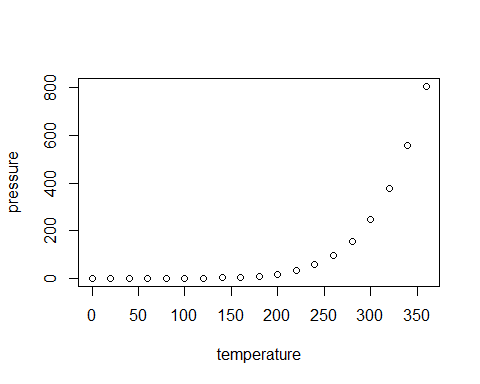
\includegraphics{Primeiro_Script_files/figure-latex/pressure-1.pdf}

Note that the \texttt{echo\ =\ FALSE} parameter was added to the code
chunk to prevent printing of the R code that generated the plot.


\end{document}
